\documentclass[12pt, twoside]{article}
\usepackage[letterpaper, margin=1in, headsep=0.5in]{geometry}
\usepackage[english]{babel}
\usepackage[utf8]{inputenc}
\usepackage{amsmath}
\usepackage{amsfonts}
\usepackage{amssymb}
\usepackage{tikz}
%\usetikzlibrary{quotes, angles}

\usepackage{graphicx}
\usepackage{enumitem}
\usepackage{multicol}

\usepackage{fancyhdr}
\pagestyle{fancy}
\fancyhf{}
\renewcommand{\headrulewidth}{0pt} % disable the underline of the header

\fancyhead[RE]{\thepage}
\fancyhead[RO]{\thepage \\ Name: \hspace{3cm}}
\fancyhead[L]{BECA / Dr. Huson / 10th Grade Geometry\\* Unit 4: Triangle Congruence\\13 December 2018}

\begin{document}
\subsubsection*{Test: Triangles, transformations, proof}
  \begin{enumerate}

    \item In  $\triangle ABC$ shown below, $m\angle A=(3x+4)^\circ$, $m\angle B=(5x-15)^\circ$, and $m\angle C=(x-7)^\circ$. What is $m\angle A$?\\[0.5cm]
        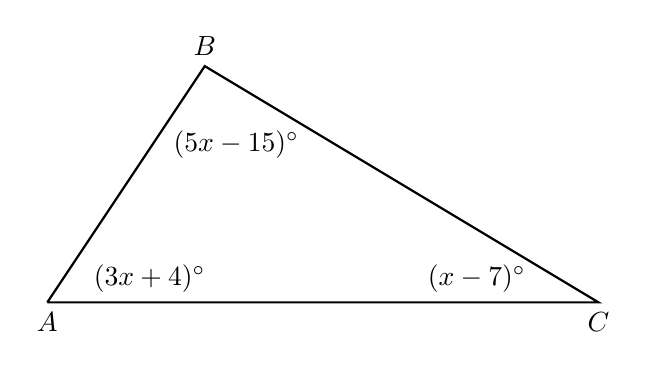
\begin{tikzpicture}
          \draw [thick]
            (2,0)node[below]{$A$}--
            (9,0)node[below]{$C$}--
            (4,3)node[above]{$B$} --(2,0);
            \node at (3.3,0)[above]{$(3x+4)^\circ$};
            \node at (8.2,0)[above left]{$(x-7)^\circ$};
            \node at (4.4,2.3)[below]{$(5x-15)^\circ$};
        \end{tikzpicture} \vspace{4cm}

    \item Given two parallel lines and a transversal, as shown below.
      \begin{center}
      \begin{tikzpicture}
        \draw [<->, thick] (1,2)--(9,2);
        \draw [<->, thick] (0,0)--(8,0);
        \draw [<->, thick] (4,-1)--(5.5,3);
        \node at (4.5,0.3) [left]{$5$};
        \node at (4.5,0.3) [right]{$6$};
        \node at (4.3,-0.3) [left]{$7$};
        \node at (4.3,-0.3) [right]{$8$};
        \node at (5.2,2) [above left]{$1$};
        \node at (5.2,2) [above right]{$2$};
        \node at (5,2) [below left]{$3$};
        \node at (5,2) [below right]{$4$};
      \end{tikzpicture}
      \end{center}
      \begin{enumerate}
        \item State the angle corresponding with $\angle 5$. \vspace{1cm}
        \item Given $m\angle 3 = 78^\circ$ and $m\angle 5 = 3x^\circ$. Find $x$. \vspace{3.5cm}
        \item In a proof, what reason would justify $\angle 3 \cong \angle 6$? \rule{6cm}{0.15mm}
      \end{enumerate}

\newpage

    \item Given $\triangle ABC$ and $\triangle DEC$ with $\angle B \cong \angle E$. $C$ is the midpoint $\overline{BE}$.\\ Prove $\triangle ABC \cong \triangle DEC$.\\[0.5cm]
       \begin{tikzpicture}
           \draw [thick]
             (-1,2)node[right]{$B$}--
             (1,-2)node[left]{$E$}--
             (4,0)node[right]{$D$}--
             (0,0)node[below left]{$C$}--
             (-4,0)node[left]{$A$}--cycle;
         \end{tikzpicture}

       \begin{multicols}{2}
         \underline{Statement} \\
         \underline{Reason}
       \end{multicols}
       \begin{multicols}{2}
         \raggedcolumns
         \begin{enumerate}[label={\arabic*)}]
           \item \rule{4cm}{0.15mm} \vspace{0.3cm}
           \item \rule{4cm}{0.15mm} \vspace{0.3cm}
           \item \rule{4cm}{0.15mm} \vspace{0.3cm}
           \item $\angle BCA \cong \angle ECD$  \vspace{0.3cm}
           \item \rule{4cm}{0.15mm} \vspace{0.3cm}
           \item $\triangle ABC \cong \triangle DEC$ \vspace{0.3cm}
         \end{enumerate}
         \begin{enumerate}[label={\arabic*)}]
           \item Given \vspace{0.3cm}
           \item Given \vspace{0.3cm}
           \item Given \vspace{0.3cm}
           \item \rule{4cm}{0.15mm} \vspace{0.3cm}
           \item Definition of a midpoint \vspace{0.3cm}
           \item \rule{4cm}{0.15mm} \vspace{0.3cm}
         \end{enumerate}
       \end{multicols} %\vspace{0.5cm}

     \item Given $m\angle K=38^\circ$ and $m\angle KNL=111^\circ$. Find $m\angle M$.\\[1cm]
       \begin{tikzpicture}
         %\draw [->, thick] (0,0)--(5,5);
         \draw [<-, thick] (8,0)--(0,0)--(3,3)--(4.5,0);
         \draw [fill] (0,0) circle [radius=0.05] node[below]{$M$};
         \draw [fill] (4.5,0) circle [radius=0.05] node[below]{$N$};
         \draw [fill] (3,3) circle [radius=0.05] node[right]{$K$};
         \draw [fill] (7,0) circle [radius=0.05] node[below]{$L$};
       \end{tikzpicture}
       \vspace{3cm}

\newpage

    \item On the graph below, draw $\overline{AB}$, with $A(-2,1)$ and $B(6,3)$, labeling the end points. Determine and state the coordinates of the midpoint $M$ of $\overline{AB}$ and mark and label it on the graph.\\
      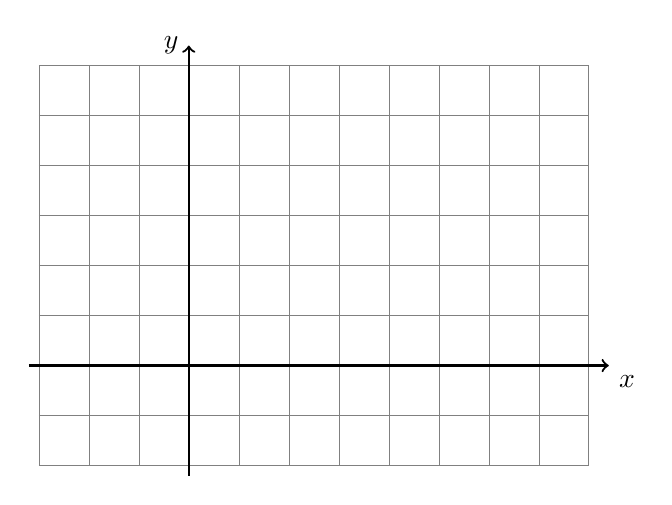
\begin{tikzpicture}[scale=.635]
        \draw [help lines] (-3,-2) grid (8,6);
        \draw [thick, ->] (-3.2,0) -- (8.4,0) node [below right] {$x$};
        \draw [thick, ->] (0,-2.2)--(0,6.4) node [left] {$y$};
      \end{tikzpicture}


      \item Express the result to the nearest thousandth.  %\vspace{0.5cm}
        \begin{multicols}{2}
          \begin{enumerate}
            \item $\sin 60^\circ = $ \vspace{0.5cm}
            \item $\cos 23^\circ =$
            \item $\tan 45^\circ = $ \vspace{0.5cm}
            \item $\sin 81^\circ =$
          \end{enumerate}
        \end{multicols}

      \item $\triangle ABC$ is shown with $m\angle C=90^\circ$. The lengths of the triangle's sides are $a$, $b$, and $c$. Express each trigonometric ratio as a fraction of two variables.
      \begin{multicols}{2}
          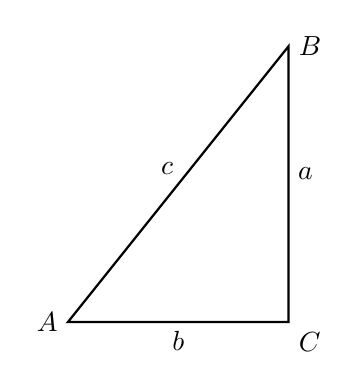
\begin{tikzpicture}[scale=0.7]
            \draw [thick]
            (0,0)node[left]{$A$}--
            (4,0)node[below right]{$C$}--
            (4,5)node[right]{$B$}--cycle;
            \node at (2,0)[below]{$b$};
            \node at (4,2.7)[right]{$a$};
            \node at (1.8,2.5)[above]{$c$};
          \end{tikzpicture}

          \begin{enumerate}
          \item $\sin A =$ \vspace{0.75cm}
          \item $\cos A =$ \vspace{0.75cm}
          \item $\tan A =$
        \end{enumerate}
    \end{multicols}

      \item Given right $\triangle JKL$ with $\overline{JK} \perp \overline{KL}$, $JL=9$, $m\angle J=29^\circ$. Find the length $JK$.
          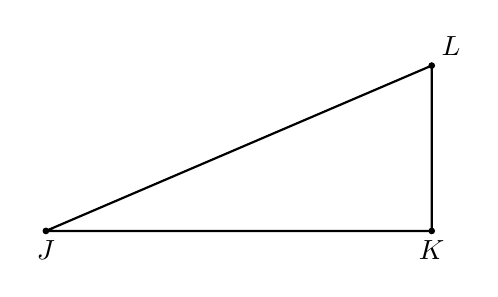
\begin{tikzpicture}[scale=0.7]
            \draw [thick](0,0)--(7,0)--(7,3)--(0,0);
            \draw [fill] (0,0) circle [radius=0.05] node[below]{$J$};
            \draw [fill] (7,0) circle [radius=0.05] node[below]{$K$};
            \draw [fill] (7,3) circle [radius=0.05] node[above right]{$L$};
          \end{tikzpicture}

\newpage

    \item Using  a  compass  and  straightedge,  construct  the  median  to  side $\overline{BC}$ in $\triangle ABC$ below.\\ (Leave all construction marks.)
      \vspace{1cm}
    \begin{center}
    \begin{tikzpicture}
      \draw [<->, thick]
        (0,0) node[left]{$A$}--
        (10,-2) node[right]{$B$}--
        (4,-5) node[below]{$C$}
        --cycle;
    \end{tikzpicture}
    \end{center}

      \vspace{2cm}

    \item With a compass and straightedge, construct a square inscribed in circle $P$. (Leave all construction marks.)
      \vspace{1cm}
      \begin{center}
      \begin{tikzpicture}
      \draw [thick] (0,0) circle [radius=4cm];
      \draw [fill] (0,0) circle [radius=0.05] node[below]{$P$};
      \end{tikzpicture}
      \end{center}

\newpage

    \item $M(5,5)$ is the midpoint of $AB$. Given $A(2,3)$, find the other endpoint, $B$. \vspace{2cm}

    \item The line $l$ has the equation $y=\frac{1}{2} x-3$.
      \begin{enumerate}
        \item What is the slope of the line $k$, given $k \parallel l$?
        \vspace{1cm}
        \item What is the slope of the line $m$, given $m \perp l$?
        \vspace{1cm}
      \end{enumerate}

    \item Given $P(3,4)$ and $Q(11,-2)$, find the length of $\overline{PQ}$.
        \vspace{4cm}

    \item Apply the translation $(x,y) \rightarrow (x-1,y+3)$ to the point $A(0,-4)$. \vspace{1cm}
    \item What is the image of $B(4,3)$ under a reflection across the $x$-axis? \vspace{1cm}
    \item State the translation that would map $C(1,5)$ onto $C'(4,3)$. \vspace{1cm}


    \item A translation maps $A(5,2) \rightarrow A'(-2,3)$. What is the image of $B(-1,5)$ under the same translation?  \vspace{0.5cm}

    \item The image of triangle $ABC$ after a translation is $\triangle A'B'C'$. Is the area of the triangle greater, smaller, or the same after the translation? Justify your answer.

\newpage

    \item In  $\triangle ABC$ shown below, side $\overline{AC}$ is extended to point $D$ with $m\angle DAB=(180-2x)^\circ$, $m\angle C=(x-10)^\circ$, and $m\angle B=(3x+10)^\circ$.
      \begin{center}
        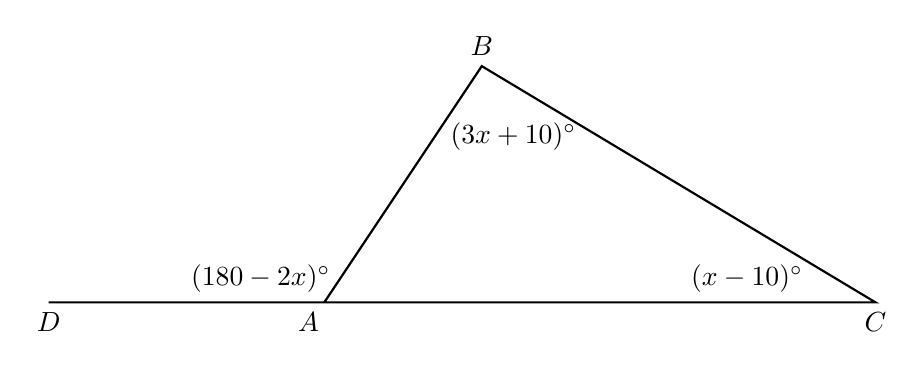
\begin{tikzpicture}
          \draw [thick](-1.5,0)node[below]{$D$}--
            (1.8,0)node[below]{$A$}--
            (9,0)node[below]{$C$}--
            (4,3)node[above]{$B$} --(2,0);
            \node at (2.2,0)[above left]{$(180-2x)^\circ$};
            \node at (8.2,0)[above left]{$(x-10)^\circ$};
            \node at (4.4,2.4)[below]{$(3x+10)^\circ$};
        \end{tikzpicture}
      \end{center}
      What is $m\angle BAC$?



  \item In the diagram below, $\overleftrightarrow{AC}$ has endpoints with coordinates $A(-3,2)$ and $C(3, -7)$.
    \begin{center} %4 quadrant regents grid
      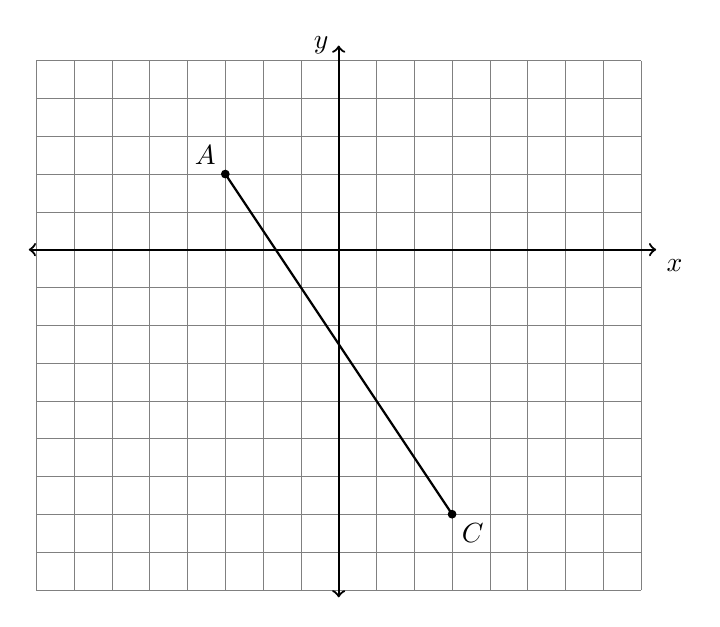
\begin{tikzpicture}[scale=.48]
        \draw [help lines] (-8,-9) grid (8,5);
        \draw [thick, <->] (-8.2,0) -- (8.4,0) node [below right] {$x$};
        \draw [thick, <->] (0,-9.2)--(0,5.4) node [left] {$y$};
        \draw [thick] (-3,2)--(3,-7);
        \draw [fill] (-3,2) circle [radius=0.1] node[above left] {$A$};
        \draw [fill] (3,-7) circle [radius=0.1] node[below right] {$C$};
      \end{tikzpicture}
    \end{center}
    If $B$ is a point on  and $AB {:} BC = 1{:}2$,  what  are  the  coordinates of $B$?

\newpage


\newpage


  \item Triangle $\triangle DAN$ is graphed on the set of axes below. The vertices of $\triangle DAN$ have the coordinates $T(-1,-2)$, $E(8,1)$, and $N(3,6)$.
    \begin{center} %4 quadrant regents grid
    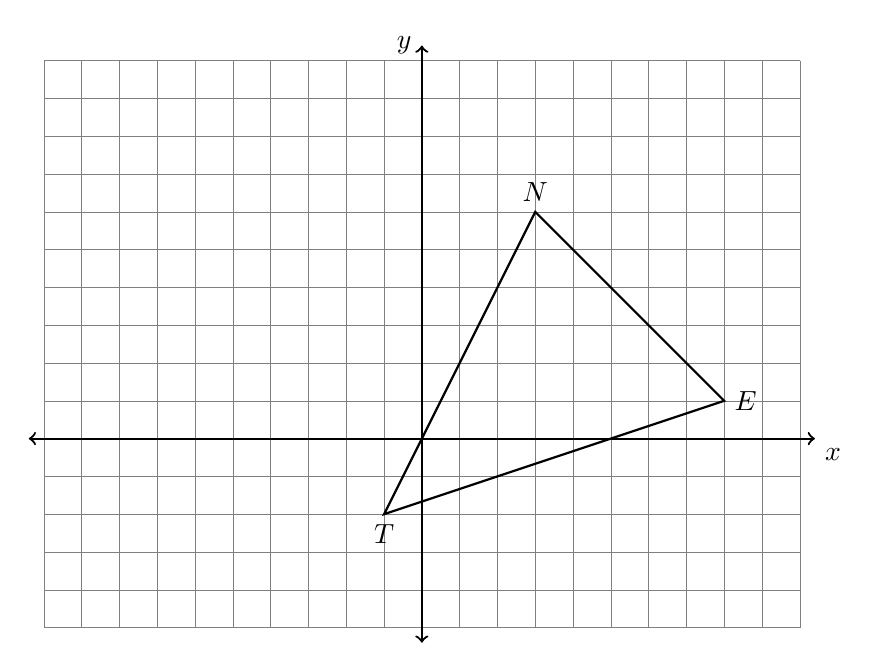
\begin{tikzpicture}[scale=.48]
      \draw [help lines] (-10,-5) grid (10,10);
      \draw [thick, <->] (-10.4,0) -- (10.4,0) node [below right] {$x$};
      \draw [thick, <->] (0,-5.4)--(0,10.4) node [left] {$y$};
      \draw [thick] (-1,-2) node[below] {$T$}--
      (8,1) node[right] {$E$}--
      (3,6) node[above] {$N$}--
      cycle;
      %\draw [fill] (5,0) circle [radius=0.1] node[above left] {$P$};
    \end{tikzpicture}
    \end{center}
    \begin{enumerate}
      \item Draw an altitude through point $N$ perpendicular to $\overline{TE}$.
      \item What is the length of the altitude drawn through $N$? \vspace{1.5cm}
      \item What is the length of the base, $TE$?  \vspace{1.5cm}
      \item Find the area of  $\triangle DAN$.
    \end{enumerate}


  \end{enumerate}

  \end{document}



  \item Given two vertical angles, $m \angle 1 = 5x+9$, $m \angle 2 = 6x-1$. Find $m \angle 1$.\\
  For full credit, check by comparing to $m\angle 2$.
      \begin{flushright}
      \begin{tikzpicture}[scale=.7]
        \draw [<->, thick] (0,-1.5)--(10,1.5);
        \draw [<->, thick] (2,3.5)--(7,-3.5);
        \node at (3,.4){1};
        \node at (6,-.6){2};
      \end{tikzpicture}
      \end{flushright}

  \item Given $\overrightarrow{BA} \perp \overrightarrow{BC}$, $m \angle ABD = 10x+15$, and $m \angle DBC = 5x$. Find $m \angle DBC$. \\[0.5cm]
  For full credit, show the check using both angle measures.
    \begin{flushleft}
    \begin{tikzpicture}[scale=1.3]
      \draw [<->, thick] (0,3)--(0,0)--(5,0);
      \draw [->, thick] (0,0)--(3.5, 2);
      \draw [-, thin] (0, 0.4)--(0.4, 0.4)--(0.4, 0);
      %\node at (3,.4){1};
      %\node at (6,-.6){2};
      \draw [fill] (0,0) circle [radius=0.05] node[below]{$B$};
      \draw [fill] (0,2) circle [radius=0.05] node[left]{$A$};
      \draw [fill] (4,0) circle [radius=0.05] node[below]{$C$};
      \draw [fill] (2.625, 1.5) circle [radius=0.05] node[below]{$D$};
    \end{tikzpicture}
    \end{flushleft}
    \vspace{3cm}

    \item Given the circle $C$ with circumference $12\pi$.
  \begin{enumerate}
    \item Write down the formula for the circumference of a circle and solve for the radius yielding a circumference of $12\pi$. \vspace{1cm}
    \item Find the area of the circle.
  \end{enumerate}
  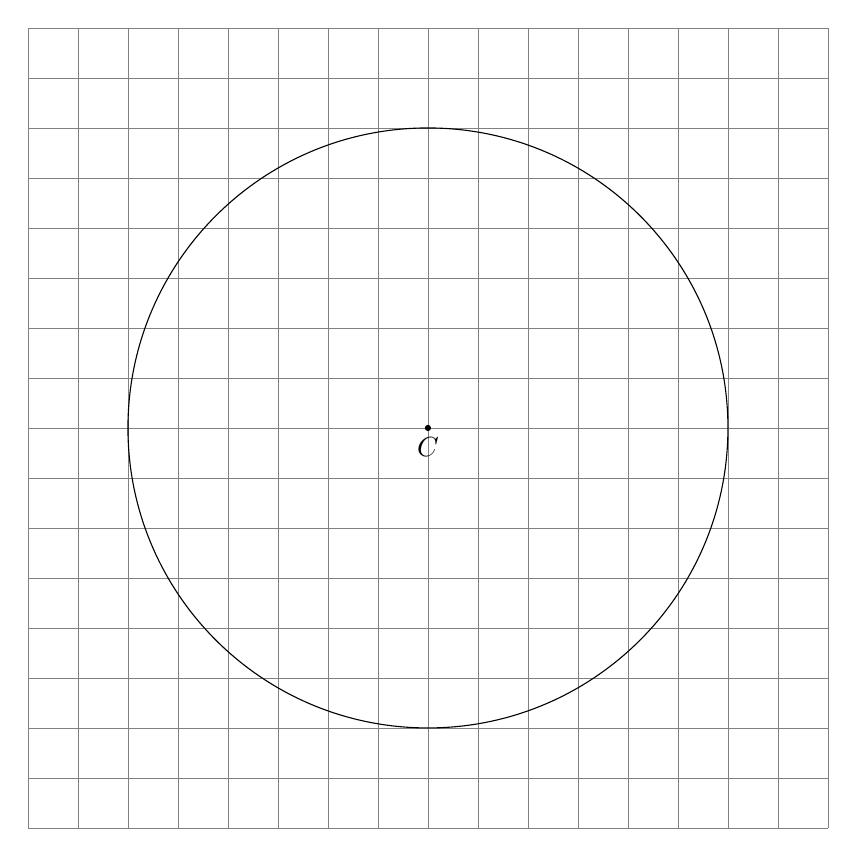
\begin{tikzpicture}[scale=.635]
    \draw [help lines] (-8,-8) grid (8,8);
    %\draw [thick, ->] (-2.2,0) -- (10.4,0) node [below right] {$x$};
    %\draw [thick, ->] (0,-2.2)--(0,10.4) node [left] {$y$};
    \draw (0,0) circle [radius=6] node[below]{$C$};
    \draw [fill] (0,0) circle [radius=0.05];
  \end{tikzpicture}

  \item On the graph, draw polygon ABCDEF with vertices A(1, 1), B(1, 4), C(3, 4), D(3, 7), E(8, 7), and F(8, 1). Find the perimeter and the area of the polygon.\\[1cm]
  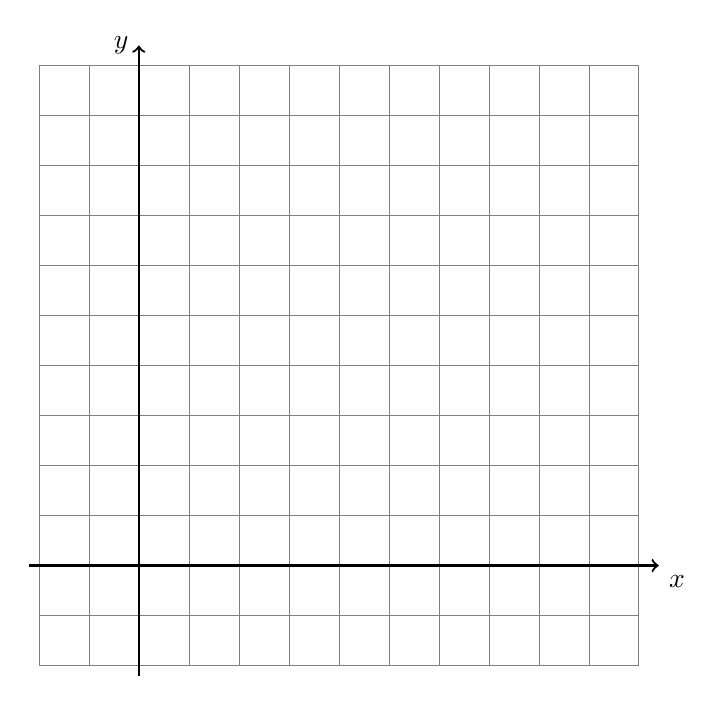
\begin{tikzpicture}[scale=.635]
    \draw [help lines] (-2,-2) grid (10,10);
    \draw [thick, ->] (-2.2,0) -- (10.4,0) node [below right] {$x$};
    \draw [thick, ->] (0,-2.2)--(0,10.4) node [left] {$y$};
  \end{tikzpicture}
  \vspace{2cm}

  \item Given a circle $O$ with radius $5$.
  \begin{enumerate}
    \item Find the circumference of $O$. \vspace{2cm}
    \item Find the area of $O$. \vspace{2cm}
  \end{enumerate}


\newpage

  \item Given $\overline{JKL}$, $JL=24$, and the point $K$ partitions $\overline{JL}$ in a ratio of 1:3.\\[0.5cm] Find ${JK}$. \\[1.5cm]
      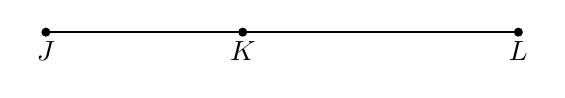
\begin{tikzpicture}
        \draw [-, thick] (1,0)--(7,0);
        \draw [fill] (1,0) circle [radius=0.05] node[below]{$J$};
        \draw [fill] (3.5,0) circle [radius=0.05] node[below]{$K$};
        \draw [fill] (7,0) circle [radius=0.05] node[below]{$L$};
      \end{tikzpicture} \vspace{3cm}
